\chapter{Implementacija i korisničko sučelje}
		
		
		\section{Korištene tehnologije i alati}
		
			\indent U izradi projekta većina digitalne komunikacije ostvarena je preko platformi WhatsApp (https://web.whatsapp.com/) i Discord (https://discord.com/). Korištene su sljedeće tehnologije i alati:
			
			\begin{itemize}
				\item \textbf{Springboot}
				\begin{itemize}
					\item open source radni okvir za kreaciju mikro-servisa, savršen za naše potrebe
					\item u njemu je izrađen backend dio projekta
					\item https://spring.io/projects/spring-boot
				\end{itemize}
				
				\item \textbf{React}
				\begin{itemize}
					\item JavaScript biblioteka za izgradnju korisničkih sučelja
					\item korišten za izradu čitavog frontenda dijela aplikacije s kojim korisnik dolazi u interakciju
					\item provjerava ispravnost podataka unesenih u obrasce
					\item https://www.reactjs.org/
				\end{itemize}
				
				\item \textbf{PostgreSQL}
				\begin{itemize}
					\item jezik u kojem je napravljena baza podataka
					\item besplatan i open source sustav za upravljanje relacijskim bazama podataka s naglaskom na mogućnosti proširivanja
					\item https://www.postgresql.org/
				\end{itemize}
			
				\item \textbf{pgAdmin}
				\begin{itemize}
					\item za upravljanje bazom podataka neovisno o backendu
					\item https://www.pgadmin.org/
				\end{itemize}
			
				\item \textbf{IntelliJ}
				\begin{itemize}
					\item IDE za javu u kojem je kodiran backend dio projekta
					\item https://www.jetbrains.com/idea/
				\end{itemize}
			
				\item \textbf{Postman}
				\begin{itemize}
					\item platforma pomoću koje su testirane backend API poveznice
					\item https://www.postman.com/
				\end{itemize}
			
				\item \textbf{Render}
				\begin{itemize}
					\item cloud platforma za izradu i besplatno hostanje web-aplikacija i stranica
					\item korišten za puštanje backenda u pogon i hostanje baze podataka
					\item https://www.render.com/
				\end{itemize}
				
				\item \textbf{Vercel}
				\begin{itemize}
					\item cloud platforma za besplatno hostanje web-stranica i servisa
					\item korišten za puštanje frontenda u pogon
					\item https://www.vercel.com/
				\end{itemize}
			
				\item \textbf{GIMP 2.10}
				\begin{itemize}
					\item uređivač slika u kojem je dizajniran logotip aplikacije i pojedini grafički prikazi u dokumentaciji
					\item https://www.gimp.org/
				\end{itemize}	
			
				\item \textbf{TeXstudio}
				\begin{itemize}
					\item integrirani uređivač za LaTeX
					\item u njemu je napisana čitava projektna dokumentacija
					\item https://www.texstudio.org/
				\end{itemize}
			
				\item \textbf{TeX Live}
				\begin{itemize}
					\item softverska distribucija za TeX s mnogobrojnim paketima i fontovima
					\item https://www.tug.org/texlive/
				\end{itemize}
			
				\item \textbf{Astah UML}
				\begin{itemize}
					\item program za uređivanje svih vrsta UML dijagrama
					\item svi dijagrami u ovom dokumentu načinjeni su u Astahu
					\item https://astah.net/products/astah-uml/
				\end{itemize}
			
				\item \textbf{GitLab}
				\begin{itemize}
					\item stranica za funkcionalno zajedničko stvaranje i uređivanje grupnog projekta
					\item https://about.gitlab.com
				\end{itemize}
			
				\item \textbf{Selenium}
				\begin{itemize}
					\item program za automatizaciju web aplikacija u svrhe testiranja
					\item korištena za testove u sljedećem poglavlju (5.2)
					\item https://www.selenium.dev
				\end{itemize}
			
				\item \textbf{Visual Studio Code}
				\begin{itemize}
					\item uređivač izvornog koda za razne programske jezike
					\item https://code.visualstudio.com/
				\end{itemize}
			\end{itemize}
			
			\eject 
		
	
		\section{Ispitivanje programskog rješenja}
			
			\textbf{\textit{dio 2. revizije}}\\
			
			 \textit{U ovom poglavlju je potrebno opisati provedbu ispitivanja implementiranih funkcionalnosti na razini komponenti i na razini cijelog sustava s prikazom odabranih ispitnih slučajeva. Studenti trebaju ispitati temeljnu funkcionalnost i rubne uvjete.}
	
			
			\subsection{Ispitivanje komponenti}
			\textit{Potrebno je provesti ispitivanje jedinica (engl. unit testing) nad razredima koji implementiraju temeljne funkcionalnosti. Razraditi \textbf{minimalno 6 ispitnih slučajeva} u kojima će se ispitati redovni slučajevi, rubni uvjeti te izazivanje pogreške (engl. exception throwing). Poželjno je stvoriti i ispitni slučaj koji koristi funkcionalnosti koje nisu implementirane. Potrebno je priložiti izvorni kôd svih ispitnih slučajeva te prikaz rezultata izvođenja ispita u razvojnom okruženju (prolaz/pad ispita). }
			
			
			
			
			
			\subsection{Ispitivanje sustava}
			
			 
			 
		 	
		 	\indent U nastavku su priloženi testovi za ispitivanje sustava u radnom okviru Selenium. Testni slučajevi su napravljeni uz pomoć dodatka za preglednik Selenium IDE. Provedeni su testovi za točnu registraciju, krivu prijavu, odjavu sa profila, dodavanje događaja, te adminove mogućnosti suspendiranja i odsuspendiranja korisnika.
		 	
		 	\indent Za test točne registracije koriste se ulazni podaci "registracija1" za korisničko ime, "registracija1" za nadimak, "registracija1@gmail.com" za e-mail, te "registracija1" za lozinku i ponovljenu lozinku(prije registracije ne postoji korisnik sa istim podacima). Nakon toga se stisne gumb registriraj nakon kojeg su podaci spremljeni i moramo se vratiti na stranicu prijava. Tamo upišemo "registracija1" u polja korisničko ime i zaporka i onda uspješno ulazimo na početnu stranicu.
		 	\begin{figure}[H]
		 		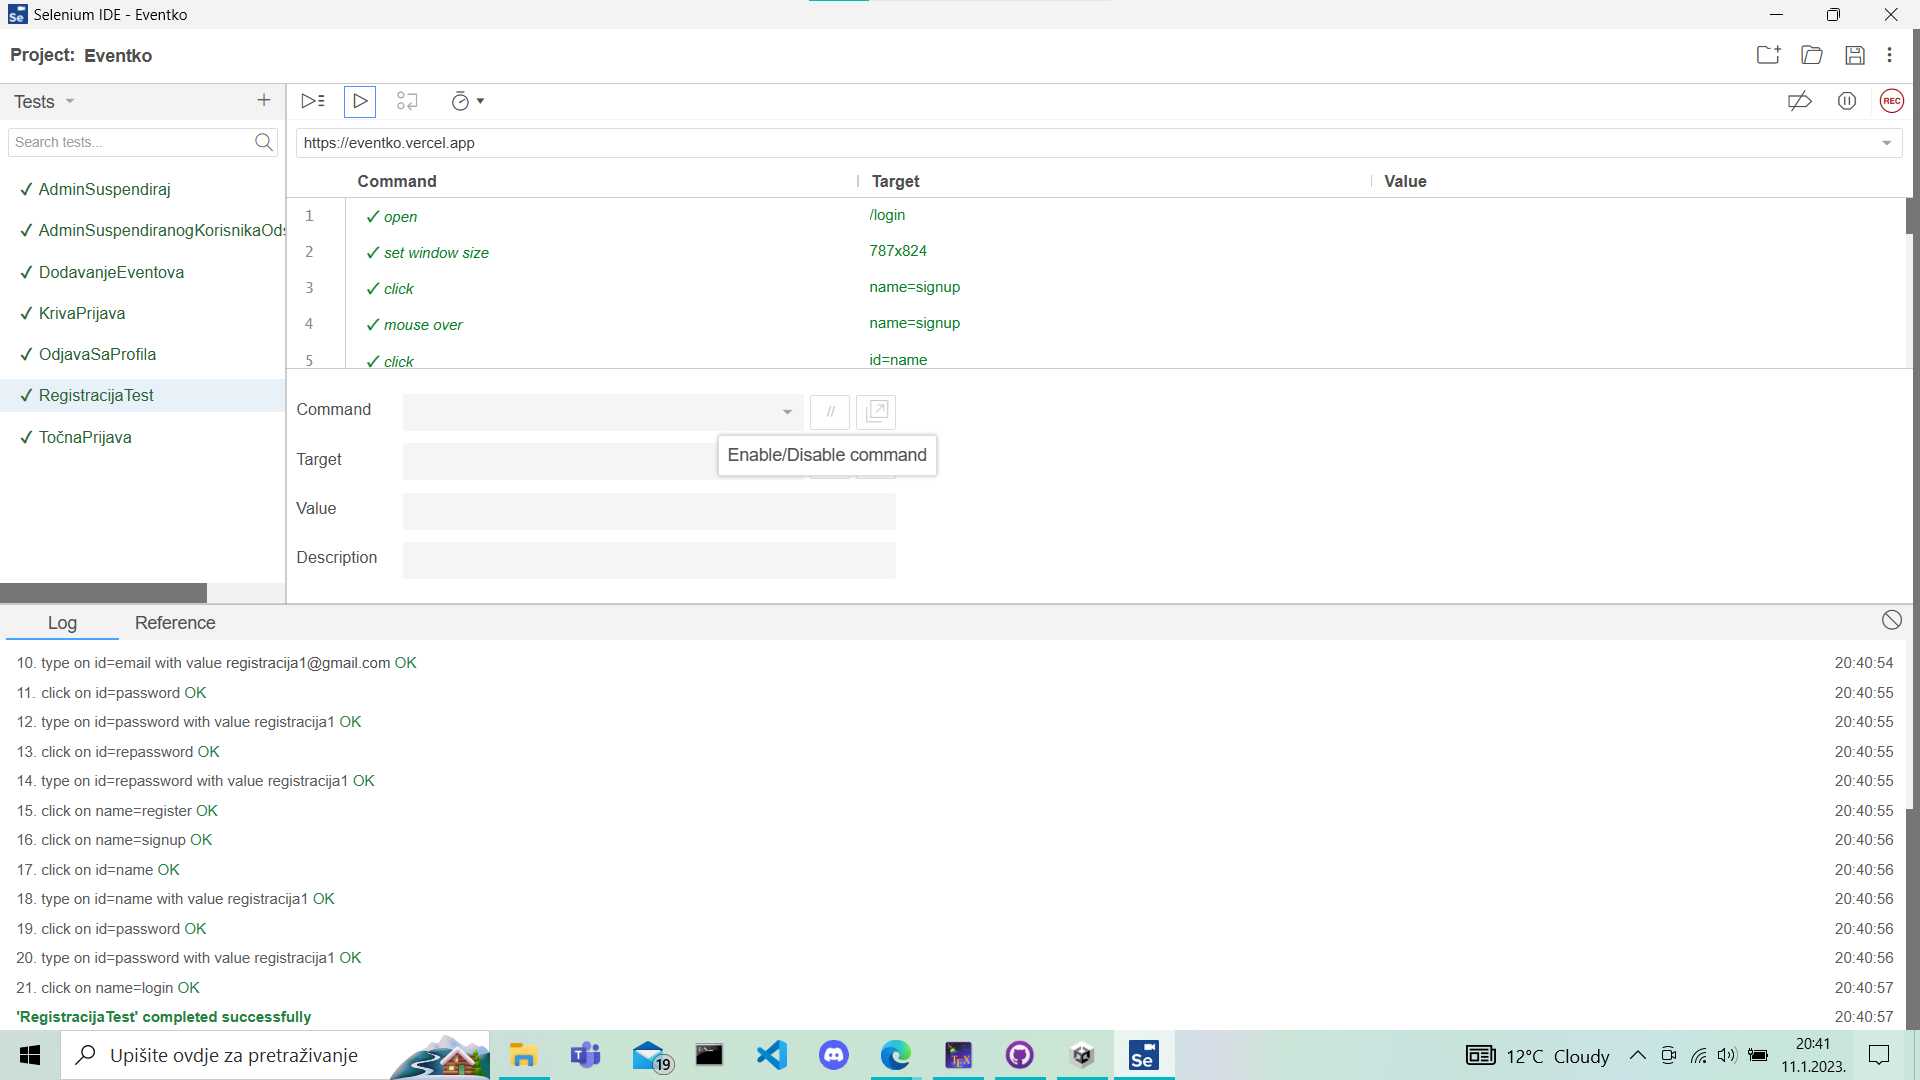
\includegraphics[width=\textwidth]{Slike/RegistracijaTest.png}
		 		\caption{Točna registracija}
		 	\end{figure}
	 	
	 		\indent Za test krive prijave koriste se ulazni podaci "VIDOJE" za korisničko ime i "VIDOJE" za zaporku(za vrijeme prijave ne postoji korisnik sa istim podacima). Pritiskom na gumb prijavi pojavljuje se poruka "Neuspješna prijava" koja se može vidjeti na drugoj slici.
	 		
	 		\begin{figure}[H]
	 			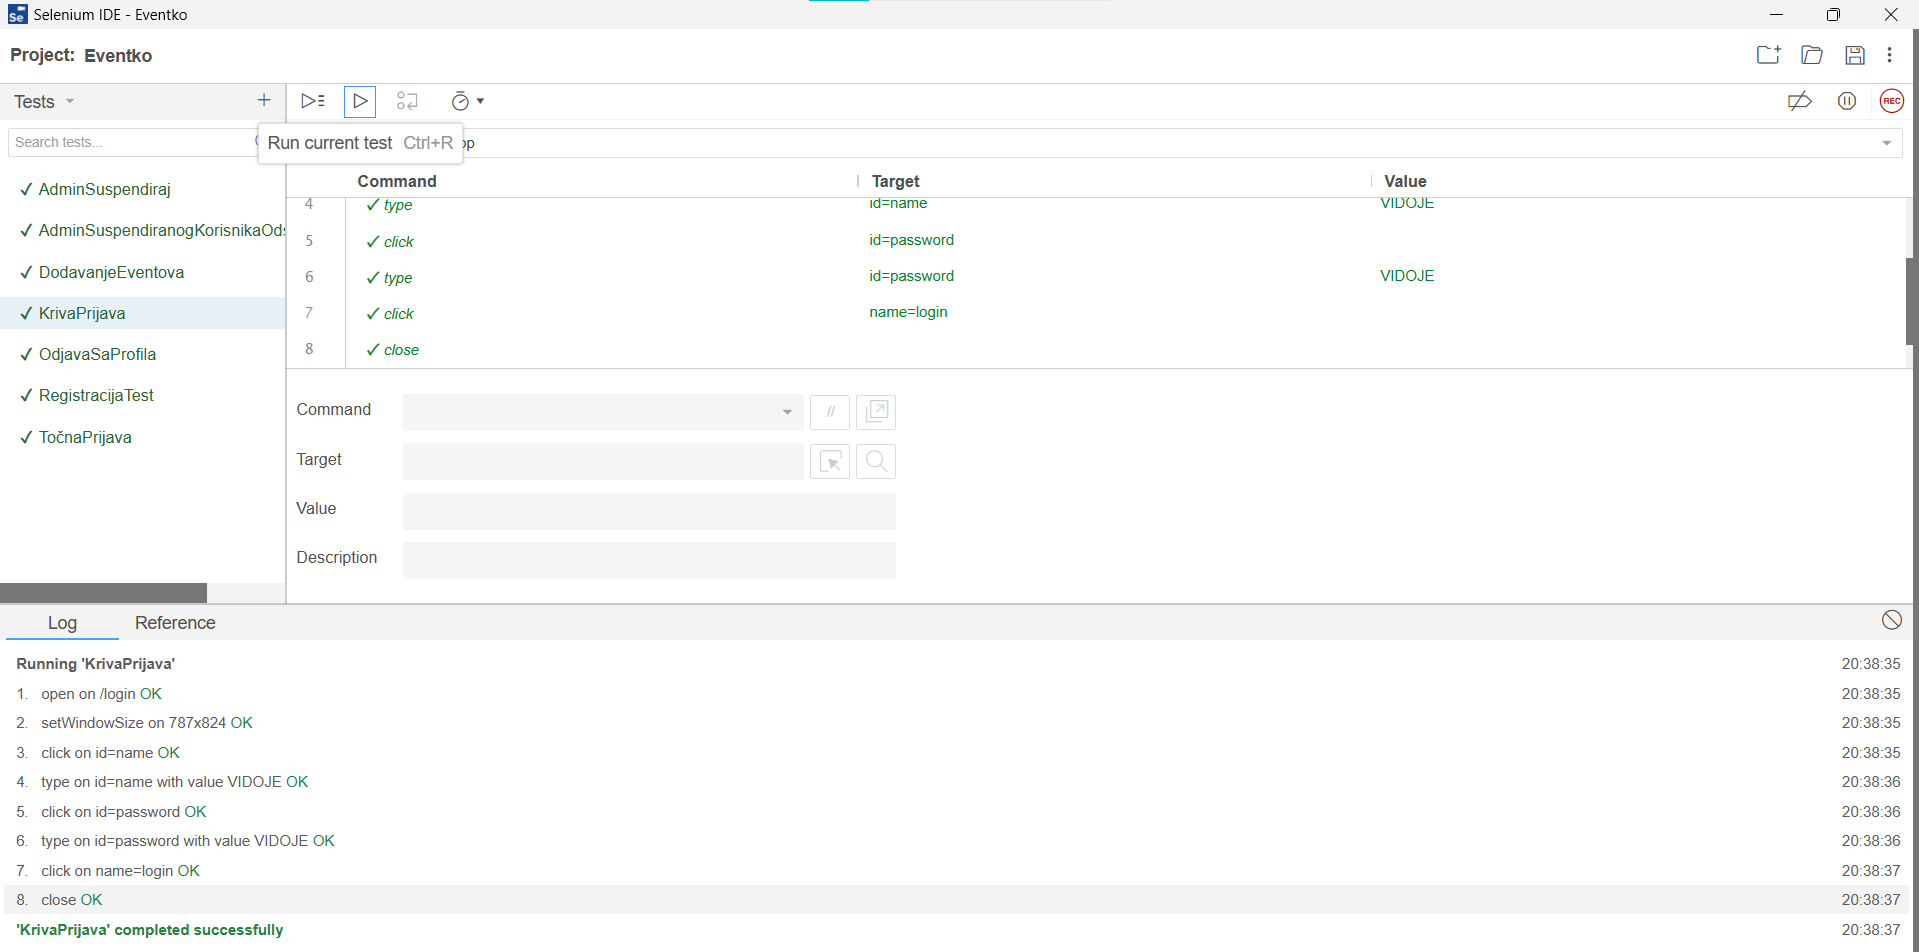
\includegraphics[width=\textwidth]{Slike/KrivaPrijava.png}
	 			\caption{Krivi podaci za prijavu}
	 		\end{figure}
 		
 			\begin{figure}[H]
 				\includegraphics[width=\textwidth]{Slike/Neuspješna prijava.png}
 				\caption{Neuspješna prijava}
 			\end{figure}
 		
 			\indent Za test odjave sa profila koriste se ulazni podaci "admin" za korisničko ime i "1234" za zaporku(postoji korisnik sa upisanim ulaznim podacima). Nakon toga se nalazimo na početnoj stranici te stisnemo tekst "Odjava" u desnom gornjem kutu i vraćeni smo na stranicu za prijavu.
 			
 			\begin{figure}[H]
 				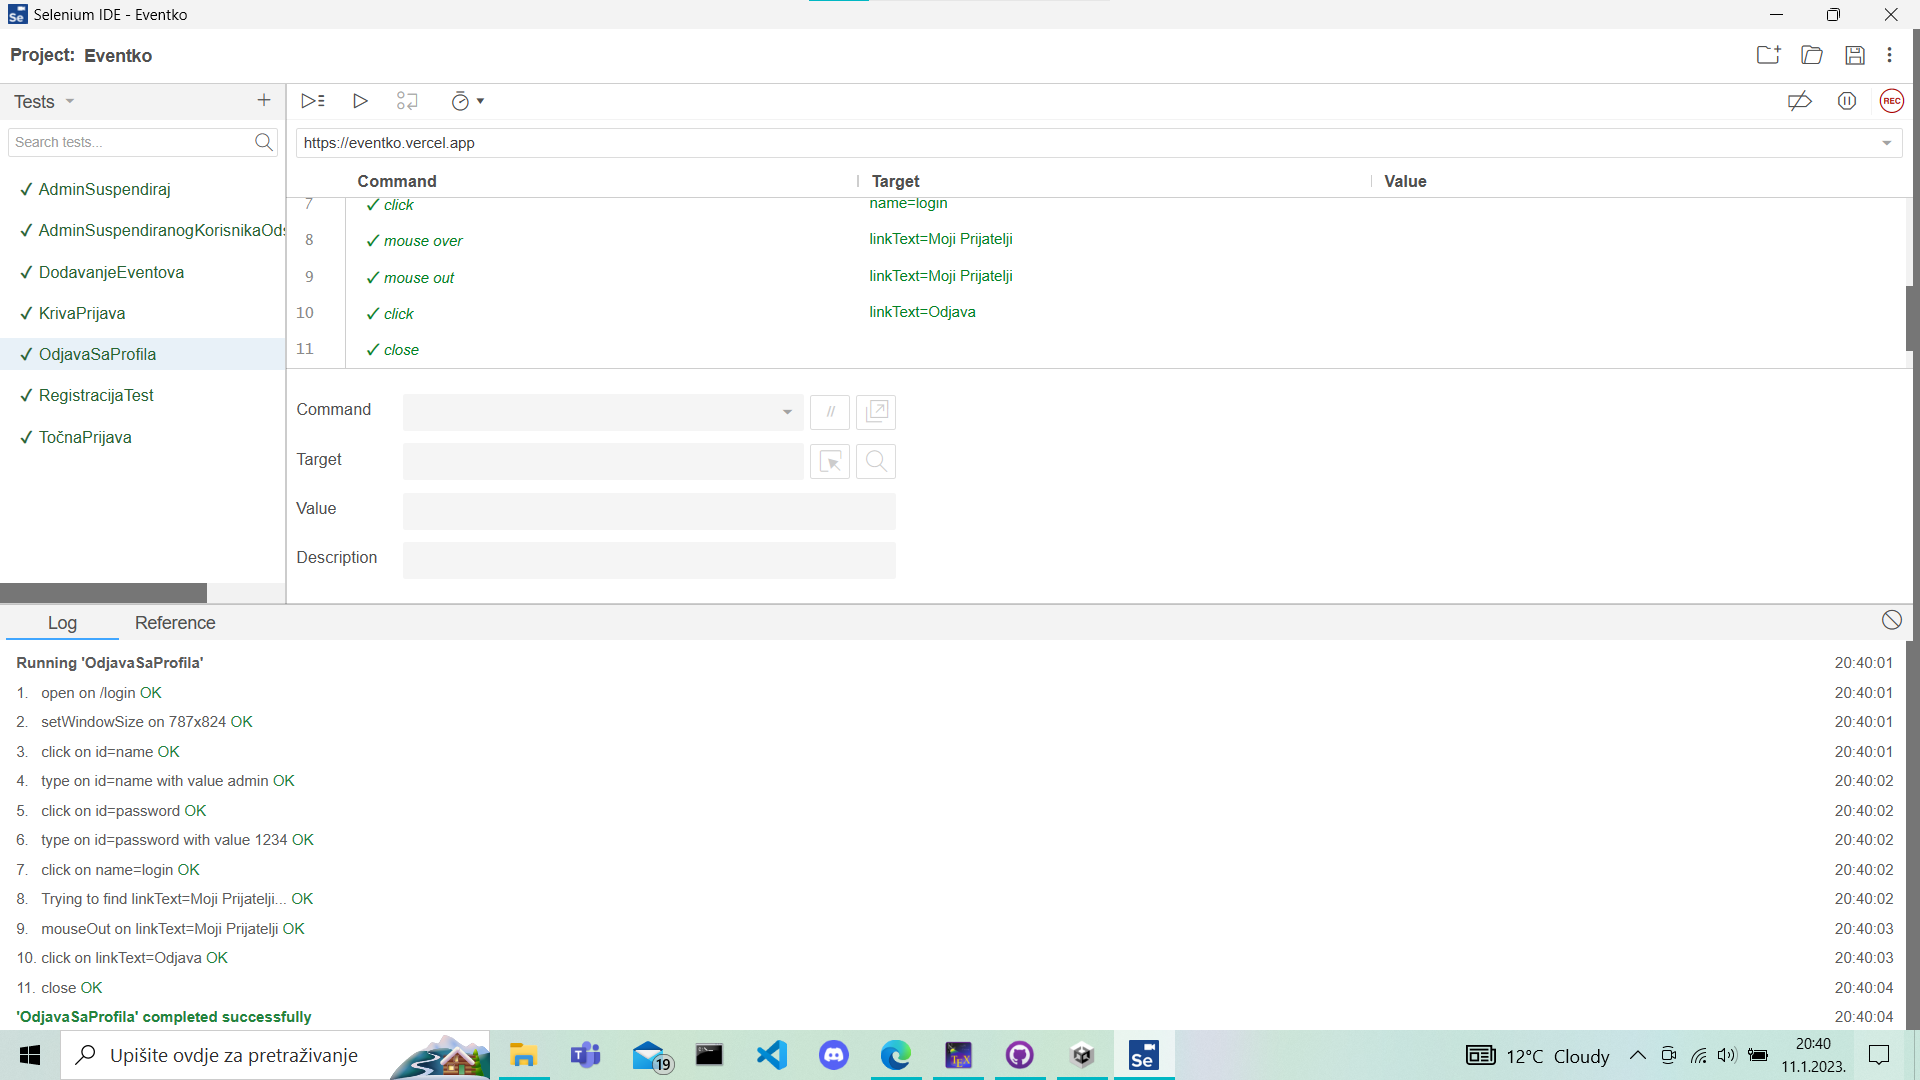
\includegraphics[width=\textwidth]{Slike/OdjavaSaProfila.png}
 				\caption{Odjava sa profila}
 			\end{figure}
 		
 			\indent Za test dodavanja događaja koriste se ulazni podaci "admin" za korisničko ime i "1234" za zaporku(postoji korisnik sa upisanim ulaznim podacima). Nakon toga se nalazimo na početnoj stranici te stisnemo "Dodaj u kalendar" u lijevom gornjem kutu. Nakon toga se otvara prozor za koji se koriste ulazni podaci "Event" za naziv događaja, "Zagreb" za mjesto događaja, "1.2.2023 i 20:21" se odabire za početak događaja i "2.2.2023 i 20:21" se odabire za kraj događaja, te "Javni događaj" se odabire za vrstu događaja, "Kava" se odabire za oznaku događaja i "Ucenje" za opis događaja. Stvoren je novi događaj i vidljiv je u kalendaru kao na drugoj slici.
 			\begin{figure}[H]
 				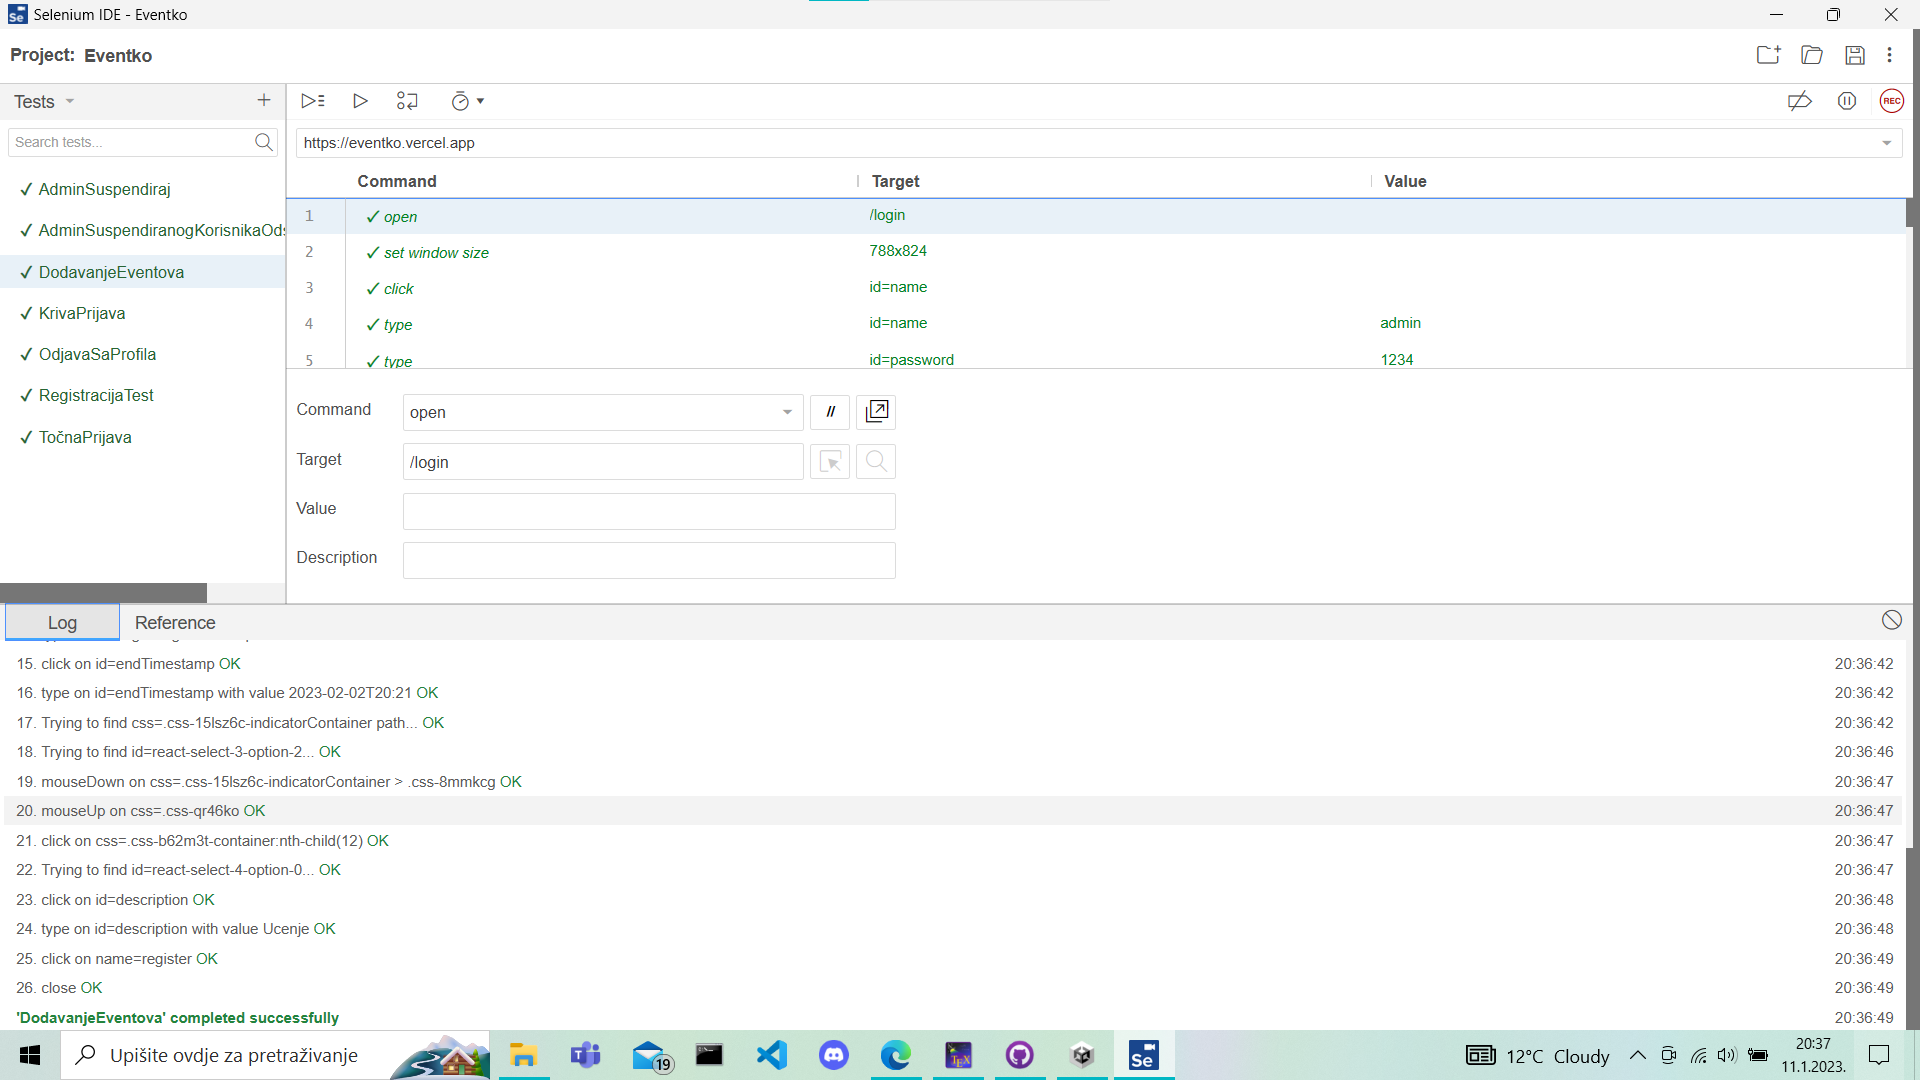
\includegraphics[width=\textwidth]{Slike/DodavanjeEventova.png}
 				\caption{Dodavanje novog događaja}
 			\end{figure}
 		
 			\begin{figure}[H]
 				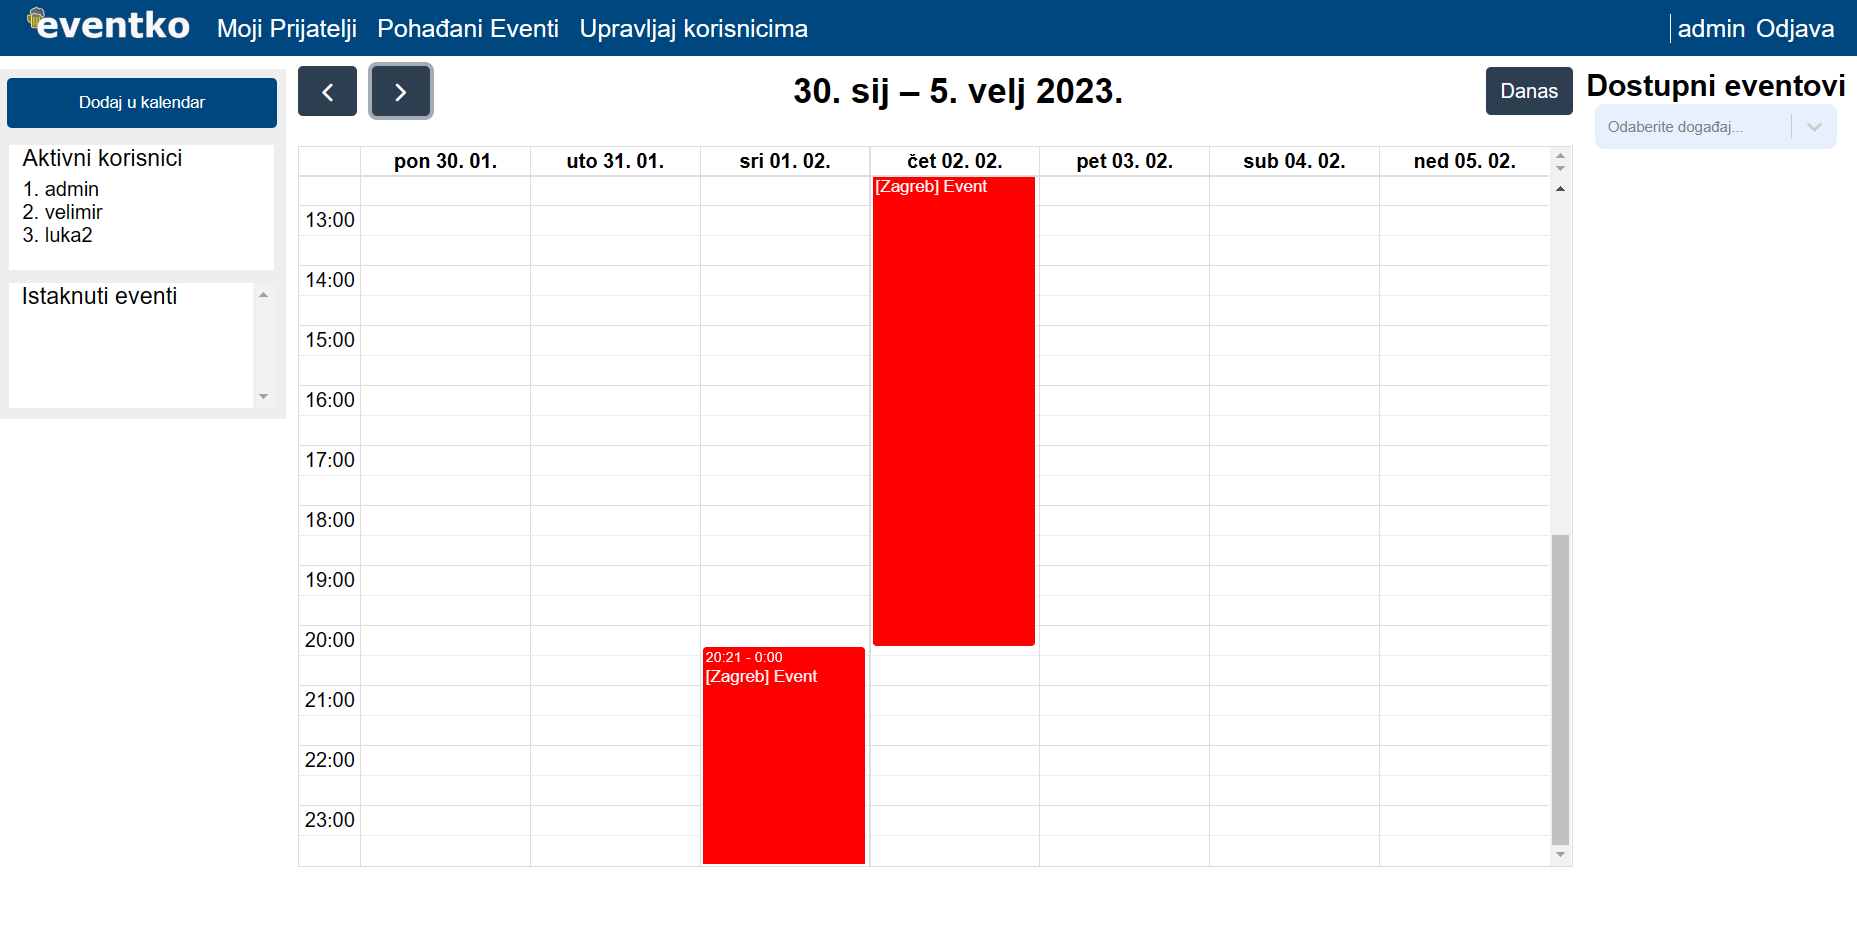
\includegraphics[width=\textwidth]{Slike/Kalendar.png}
 				\caption{Stvoren novi događaj u kalendaru}
 			\end{figure}
 			
 			\indent Za test suspendiranje korisnika koriste se ulazni podaci "admin" za korisničko ime i "1234" za zaporku(postoji korisnik sa upisanim ulaznim podacima te ima i ovlasti admina). Nakon toga se nalazimo na početnoj stranici te stisnemo "Upravljaj korisnicima". Stisnemo gumb suspendiraj i željeni korisnik je suspendiran.
 			
 			\begin{figure}[H]
 				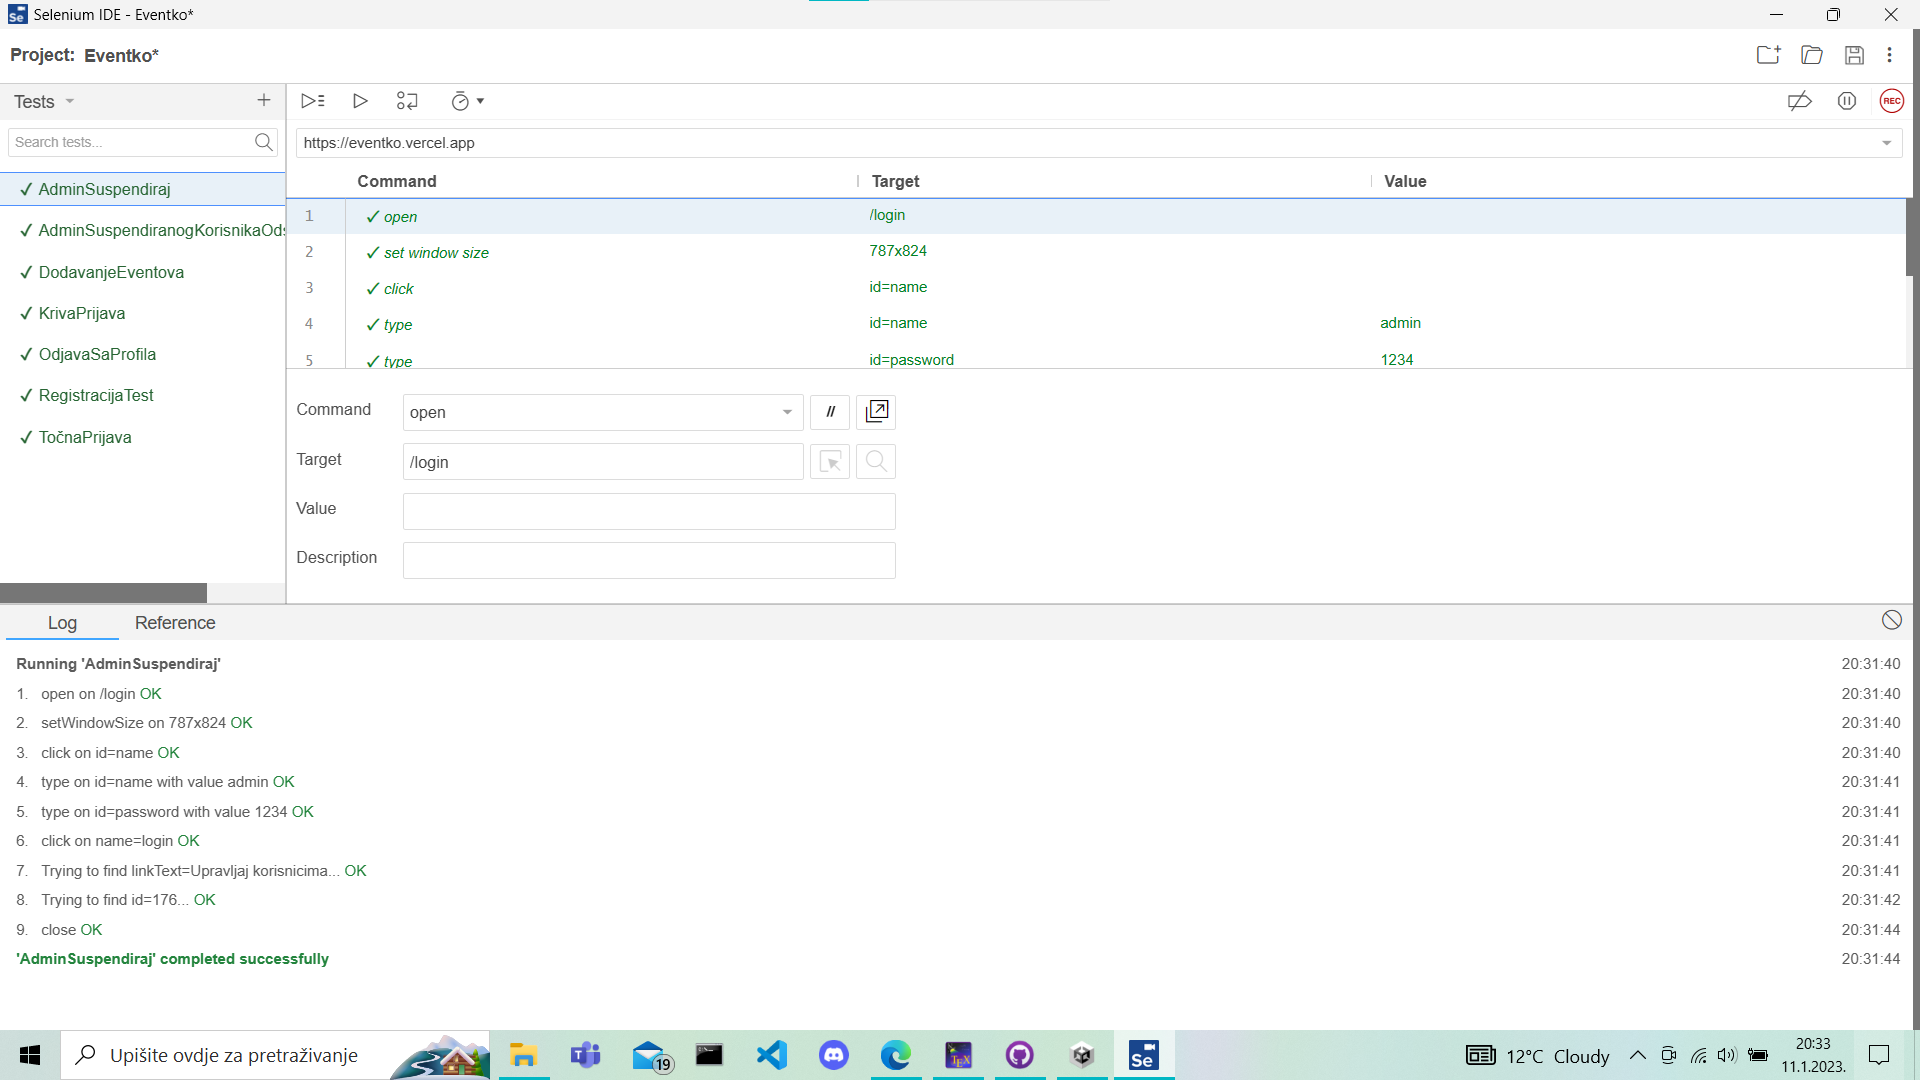
\includegraphics[width=\textwidth]{Slike/AdminSuspendirajSelenium.png}
 				\caption{Admin suspendiranje}
 			\end{figure}
 		
 		
 			\indent Za test odsuspendiranja korisnika koriste se ulazni podaci "admin" za korisničko ime i "1234" za zaporku(postoji korisnik sa upisanim ulaznim podacima te ima i ovlasti admina). Nakon toga se nalazimo na početnoj stranici te stisnemo "Upravljaj korisnicima". Stisnemo gumb odsuspendiraj i željeni korisnik je odsuspendiran.
 			
 			\begin{figure}[H]
 				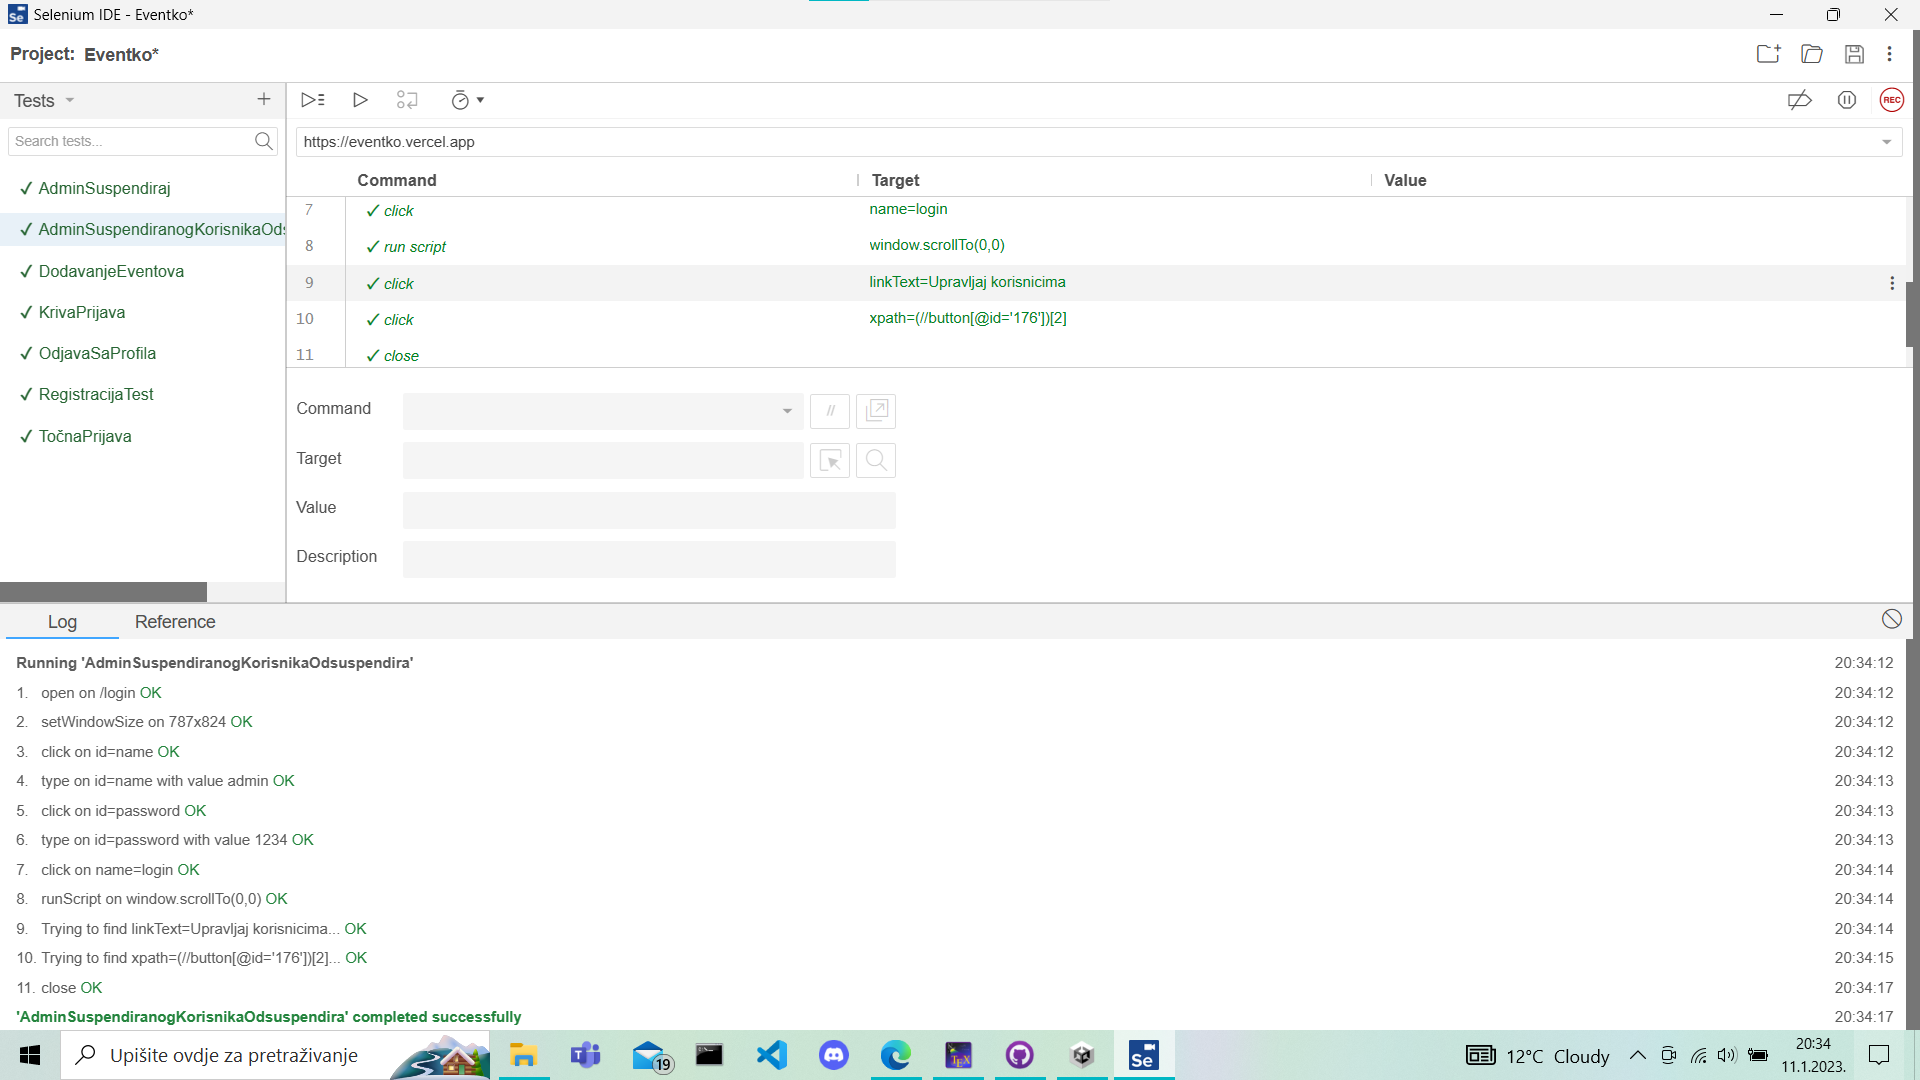
\includegraphics[width=\textwidth]{Slike/AdminSuspendiranogKorisnikaOdsuspendiraj.png}
 				\caption{Admin odsuspendiranje}
 			\end{figure}
 		
		 	
			
			\eject 
		
			
		\section{Dijagram razmještaja}
			
			 \indent Dijagram razmještaja opisuje topologiju sklopovlja i programsku potporu koja se koristi u implementaciji sustava u njegovom radnom okruženju. Na poslužiteljskom računalu se nalaze web poslužitelj na renderu i poslužitelj baze podataka na vercelu. Sustav je baziran na arhitekturi "klijent - poslužitelj", a komunikacija između računala korisnika (običan korisnik, premium korisnik, pregledavač, moderator, administrator) i poslužitelja odvija se preko HTTP veze.
			 
			 \begin{figure}[H]
			 	\includegraphics[width=\textwidth]{Dijagrami/Dijagram Razmještaja.png}
			 	\caption{Dijagram razmještaja}
			 \end{figure}
			
			\eject 
		
		\section{Upute za puštanje u pogon}
		
			\indent Puštanje web aplikacije u pogon sastoji se od tri segmenta:
			\begin{itemize}
				\item Stvaranje baze podataka
				\item Puštanje backenda u pogon
				\item Puštanje frontenda u pogon
			\end{itemize}
		
			\noindent \textbf{Stvaranje baze podataka}\\
			
			\indent Baza podataka besplatno je spremljena na web-oblaku render.com. Ona se postavlja i osposobljava sljedećim koracima:
			
			\begin{packed_enum}
				\item Stvaranje nove baze
				\begin{itemize}
					\item Za početak je potrebno (nakon registracije na render.com) odabrati opciju \textit{New} te na padajućem izborniku \textit{PostgreSQL}
					\item Pojavljuje se izbornik koji ispunjavamo kao na slici ispod
					\item Biramo \textit{Create Database}
				\end{itemize}
				\begin{figure}[H]
					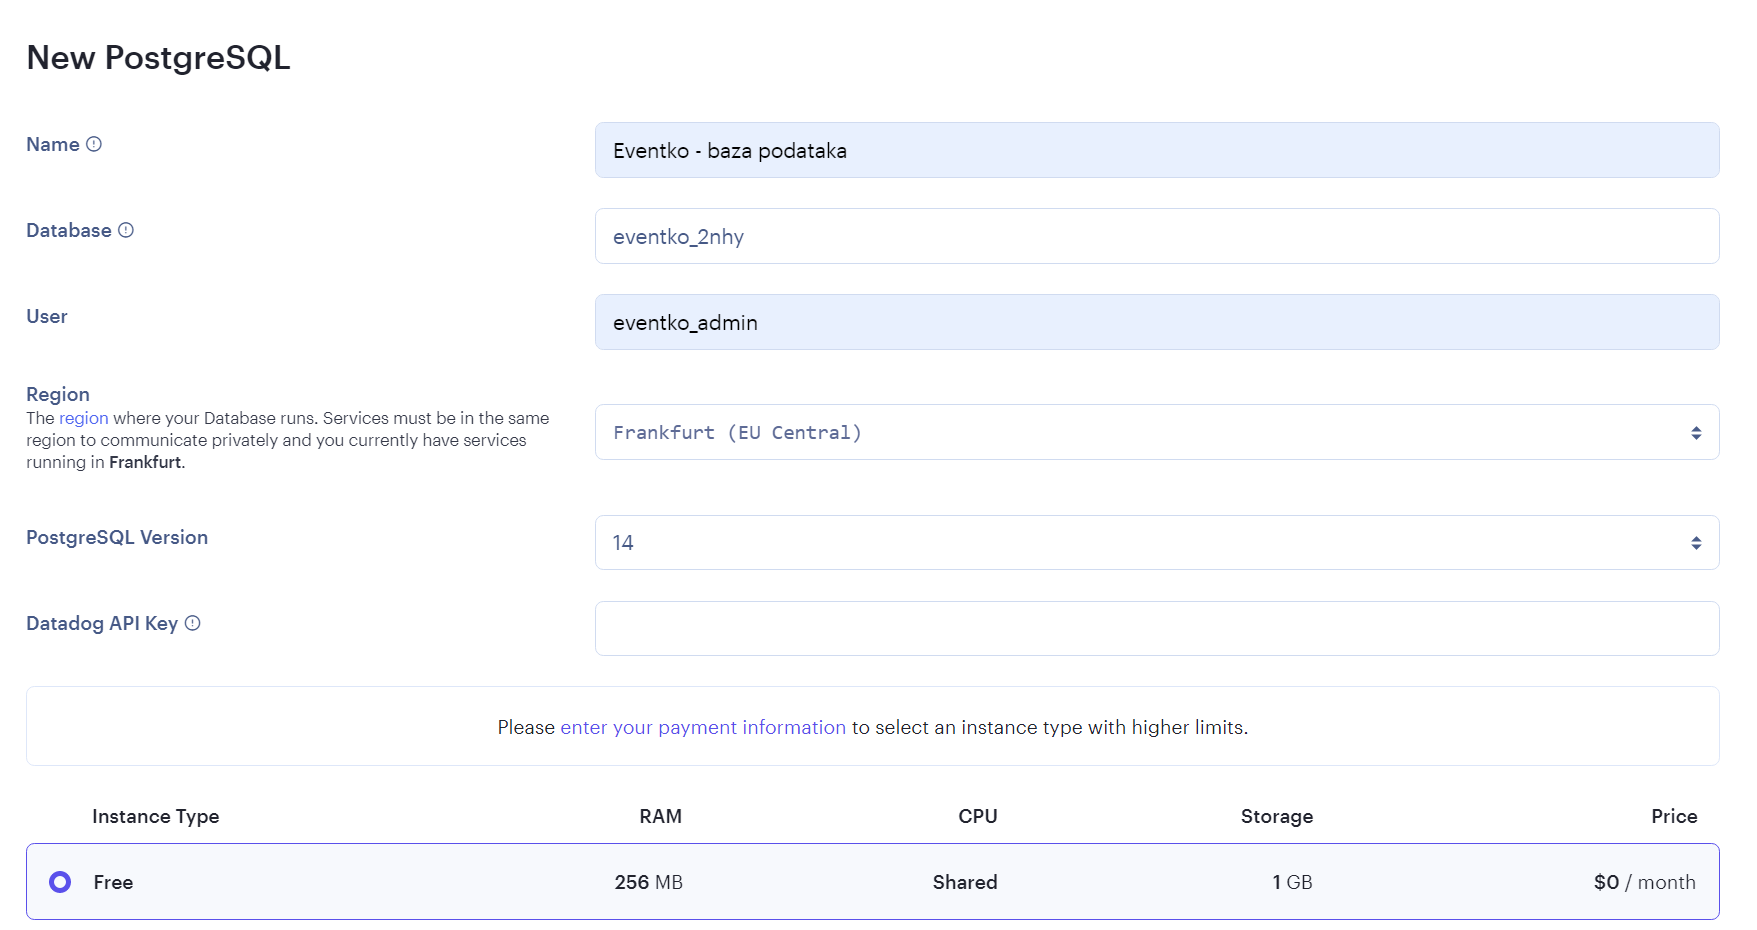
\includegraphics[width=\textwidth]{Opis deploymenta/Slika1.png}
					\caption{Stvaranje nove PostgreSQL baze}
				\end{figure}
				\eject
			
				\item Dohvat podataka za spajanje
				\begin{itemize}
					\item Redom biramo \textit{Dashboard} -> \textit{Eventko - baza podataka} -> \textit{Info}
					\item Skrolamo do izbora \textit{Connections} gdje vidimo informacije potrebne za spajanje na bazu (slika ispod).
				\end{itemize}
				\begin{figure}[H]
					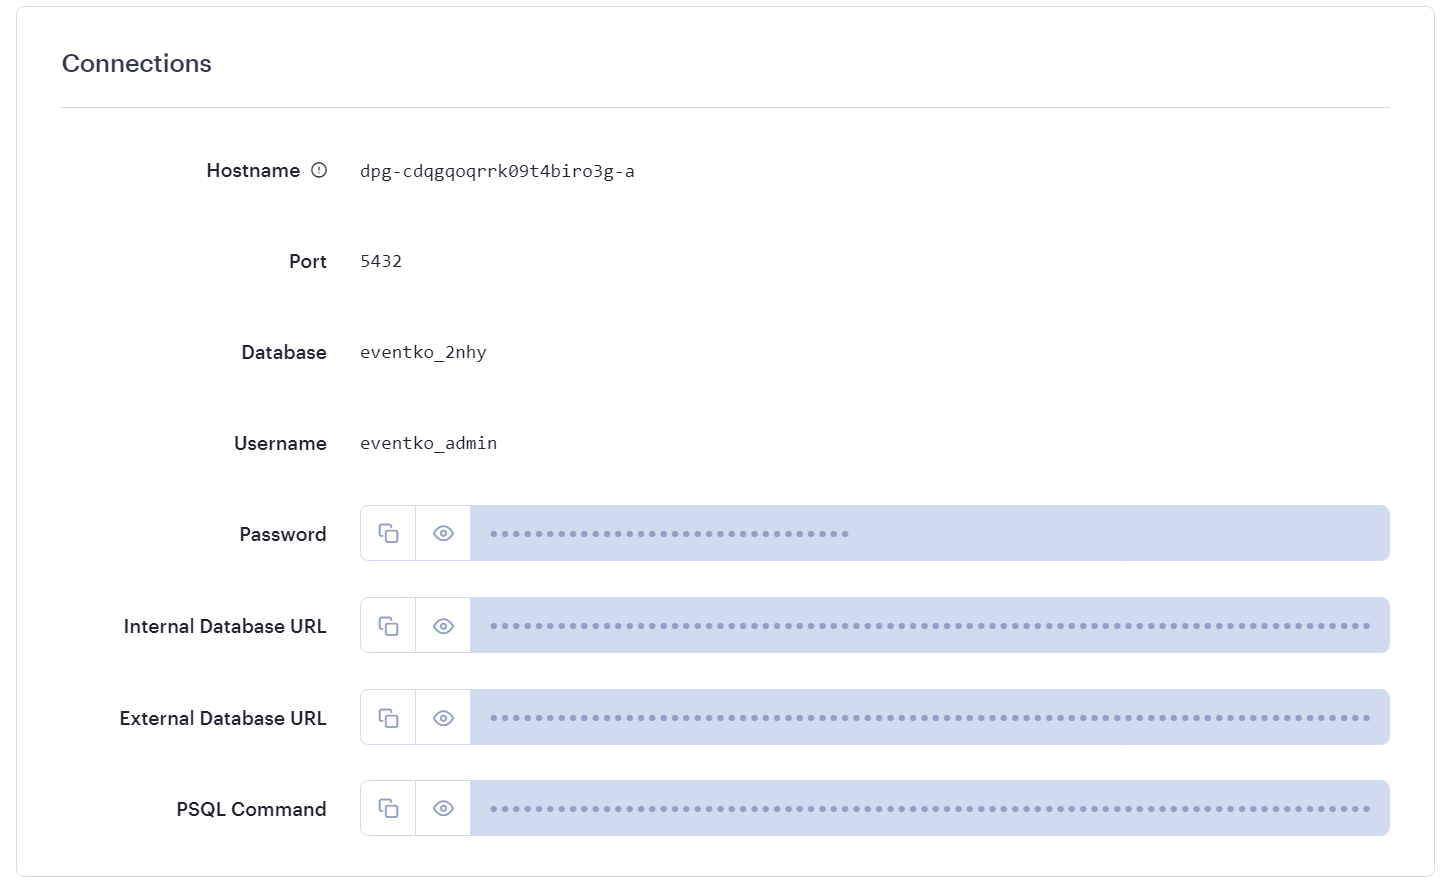
\includegraphics[width=\textwidth]{Opis deploymenta/Slika2.png}
					\caption{Dohvat podataka za spajanje baze}
				\end{figure}
			
				\item Spajanje putem pgAdmina
				\begin{itemize}
					\item Izabiremo \textit{Object} -> \textit{Create} -> \textit{Server}
					\item Na kartici \textit{General} unosimo ime servera kojeg otvaramo u pgAdminu
					\item Na kartici \textit{Connection} unosimo podatke kao na slici i spremamo ih sa \textit{Save}
				\end{itemize}
				\begin{figure}[H]
					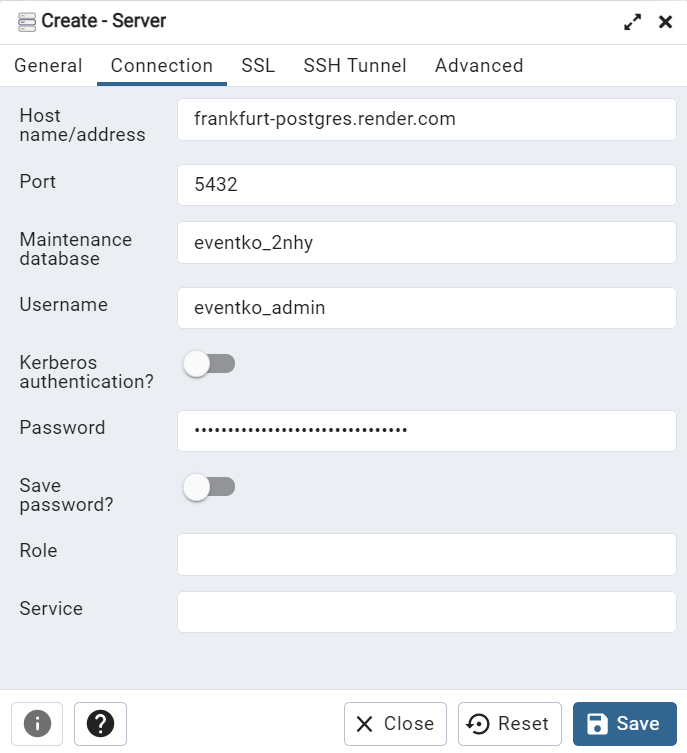
\includegraphics[width=\textwidth]{Opis deploymenta/Slika3.png}
					\caption{Unos podataka za spajanje baze}
				\end{figure}
			
				\item Spajanje iz backenda
				\begin{itemize}
					\item U src/main/resources/application.properties upisujemo naredbe sa slike
				\end{itemize}
				\begin{figure}[H]
					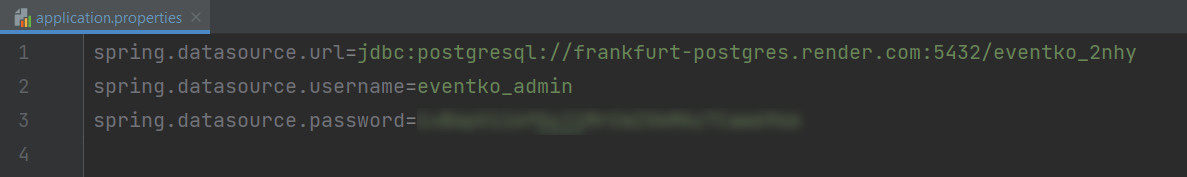
\includegraphics[width=\textwidth]{Opis deploymenta/Slika4.png}
					\caption{Spajanje baze iz backenda}
				\end{figure}
			\end{packed_enum}
			\eject
			
			\noindent \textbf{Puštanje backenda u pogon}\\
			
			\indent Backend dio projekta također koristi render.com za puštanje u pogon. Preduvjeti za to su:		\begin{itemize}
				\item Dodavanje Dockerfilea prikazanog na slici ispod
				\item Povezivanje s GitLabom na renderu
			\end{itemize}
			\begin{figure}[H]
				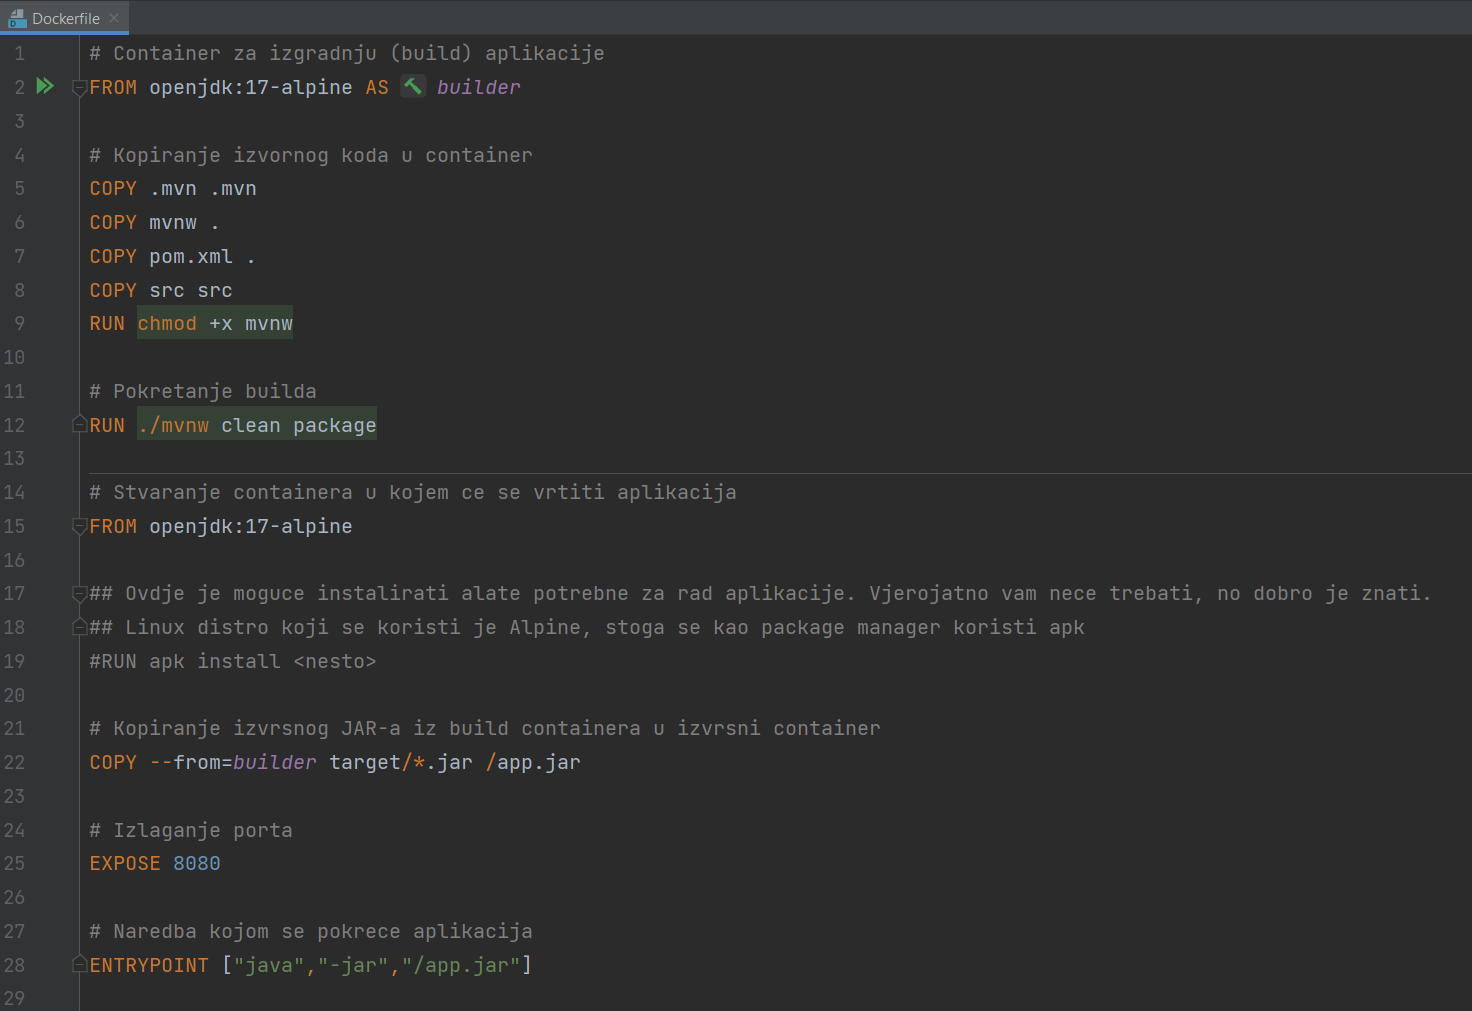
\includegraphics[width=\textwidth]{Opis deploymenta/Slika5.png}
				\caption{Potrebni Dockerfile}
			\end{figure}
		
			\indent Stvaranje backenda postižemo na sljedeći način:
			\begin{itemize}
				\item Odabiremo na render.com \textit{New} -> \textit{Web Service}
				\item Odabiremo željeni GitLab repozitorij
				\item Dalje unosimo podatke kao na slici ispod i potvrđujemo s \textit{Create Web Service}
			\end{itemize}
			\begin{figure}[H]
				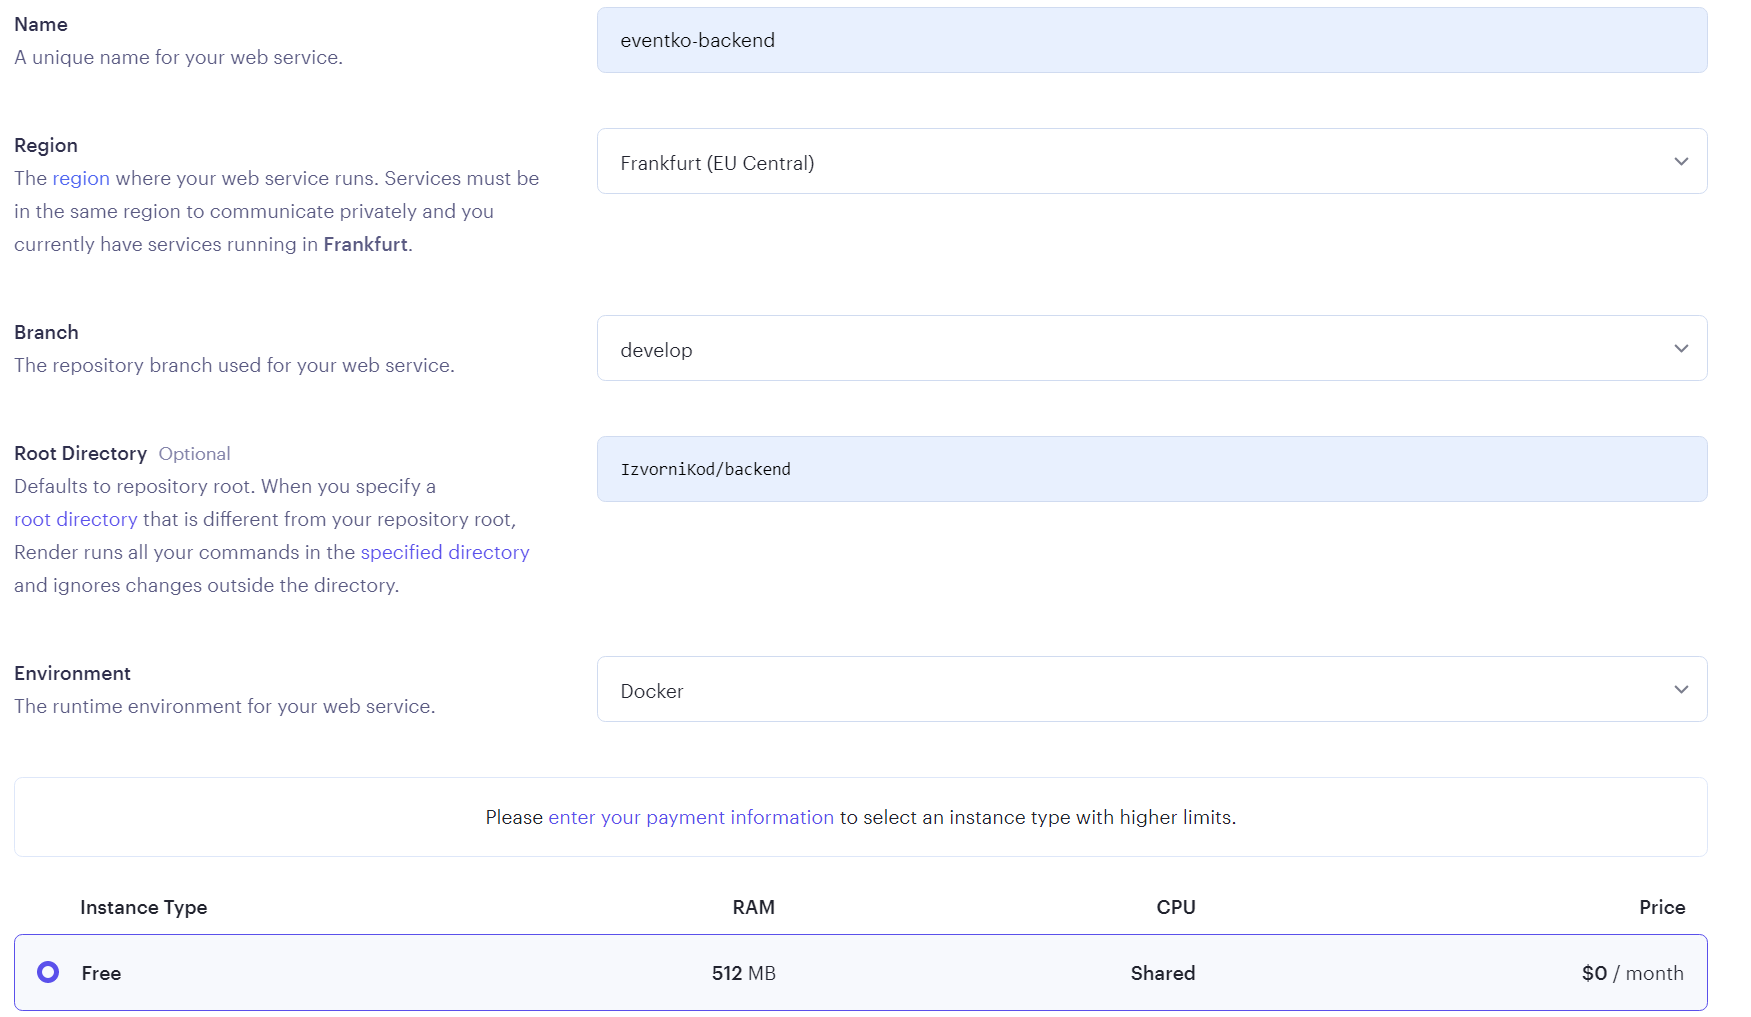
\includegraphics[width=\textwidth]{Opis deploymenta/Slika6.png}
				\caption{Stvaranje novog web servisa}
			\end{figure}
		
			\noindent \textbf{Puštanje frontenda u pogon}\\
			
			\indent Frontend dio projekta puštamo u pogon servisom vercel.com. Preduvjeti za to su:
			\begin{itemize}
				\item Dodavanje vercel.json datoteke u projekt (slika ispod) radi mapiranja putanja prema backendu
				\item Povezivanje s GitLabom i stvaranje grupe na vercelu
			\end{itemize}
		
			\begin{figure}[H]
				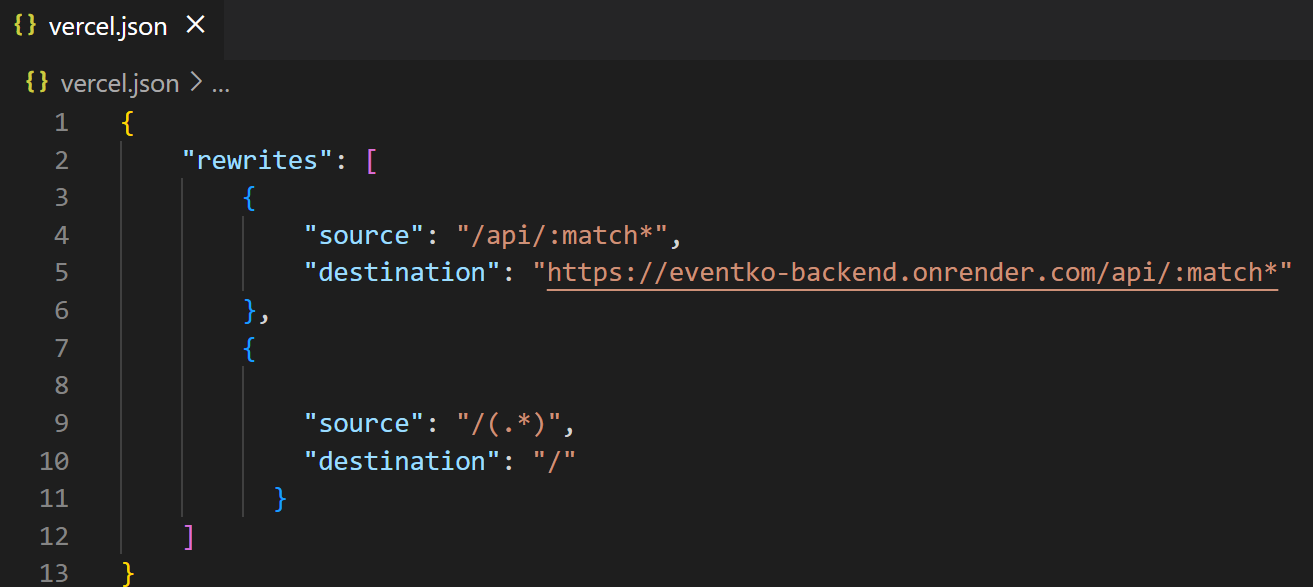
\includegraphics[width=\textwidth]{Opis deploymenta/Slika7.png}
				\caption{Potrebna vercel.json datoteka}
			\end{figure}
			\eject
			
			\indent Za puštanje frontenda u pogon provode se sljedeći koraci:
			\begin{packed_enum}
				\item Stvaranje
				\begin{itemize}
					\item Odabiremo grupu \textit{Vidoje} od ponuđenih iz našeg GitLab računa
					\item Biramo redom \textit{Add new} pa \textit{Import git repository}, pri čemu biramo repozitorij Eventko
					\item Odabiremo \textit{Configure Project}, ispunjavamo polja kao na slici ispod i završavamo s \textit{Deploy}
				\end{itemize}
				\begin{figure}[H]
					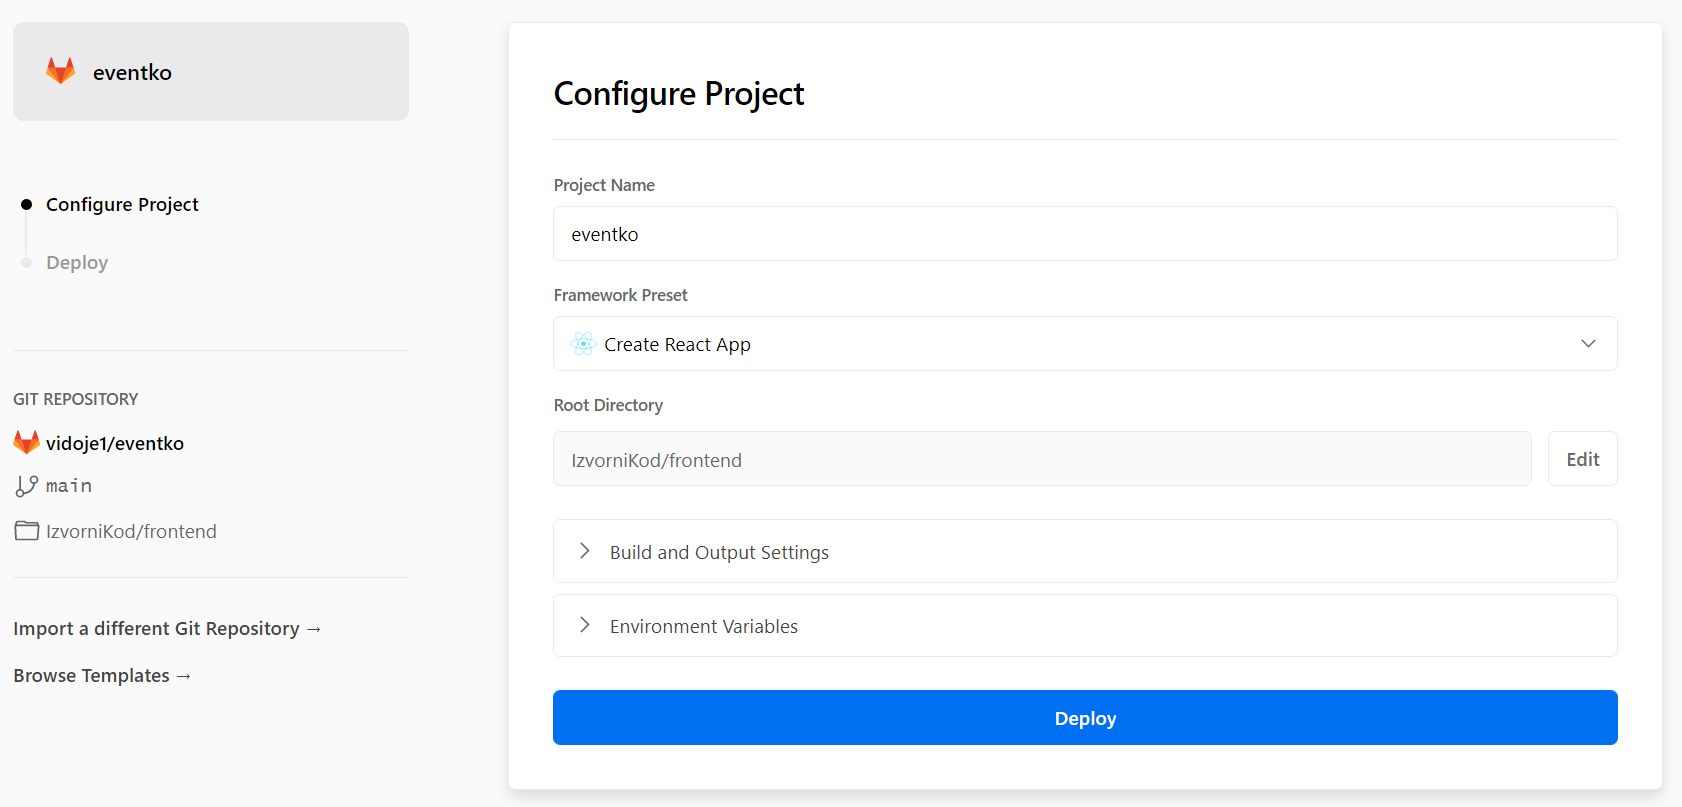
\includegraphics[width=\textwidth]{Opis deploymenta/Slika8.png}
					\caption{Stvaranje React aplikacije i puštanje u pogon}
				\end{figure}
				
				\item Promjena grane
				\begin{itemize}
					\item Biramo redom \textit{Overview} -> \textit{Eventko} -> \textit{Settings} -> \textit{Git}
					\item Mijenjamo granu iz \textit{main} u \textit{develop} kao na slici ispod te spremamo sa \textit{Save}
				\end{itemize}
				\begin{figure}[H]
					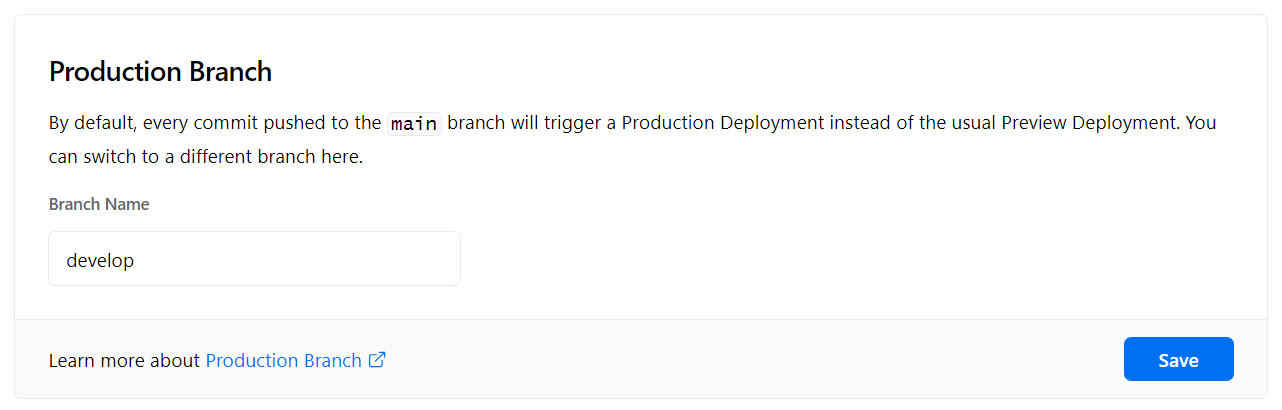
\includegraphics[width=\textwidth]{Opis deploymenta/Slika9.png}
					\caption{Promjena razvojne grane}
				\end{figure}
				\eject
				
				\item Izmjena dodijeljene domene web-stranice (opcionalno)
				\begin{itemize}
					\item Biramo redom \textit{Overview} -> \textit{Eventko} -> \textit{Settings} -> \textit{Domains}
					\item Unosimo novu željenu domenu kao na slici ispod i spremamo sa \textit{Save}
				\end{itemize}
				\begin{figure}[H]
					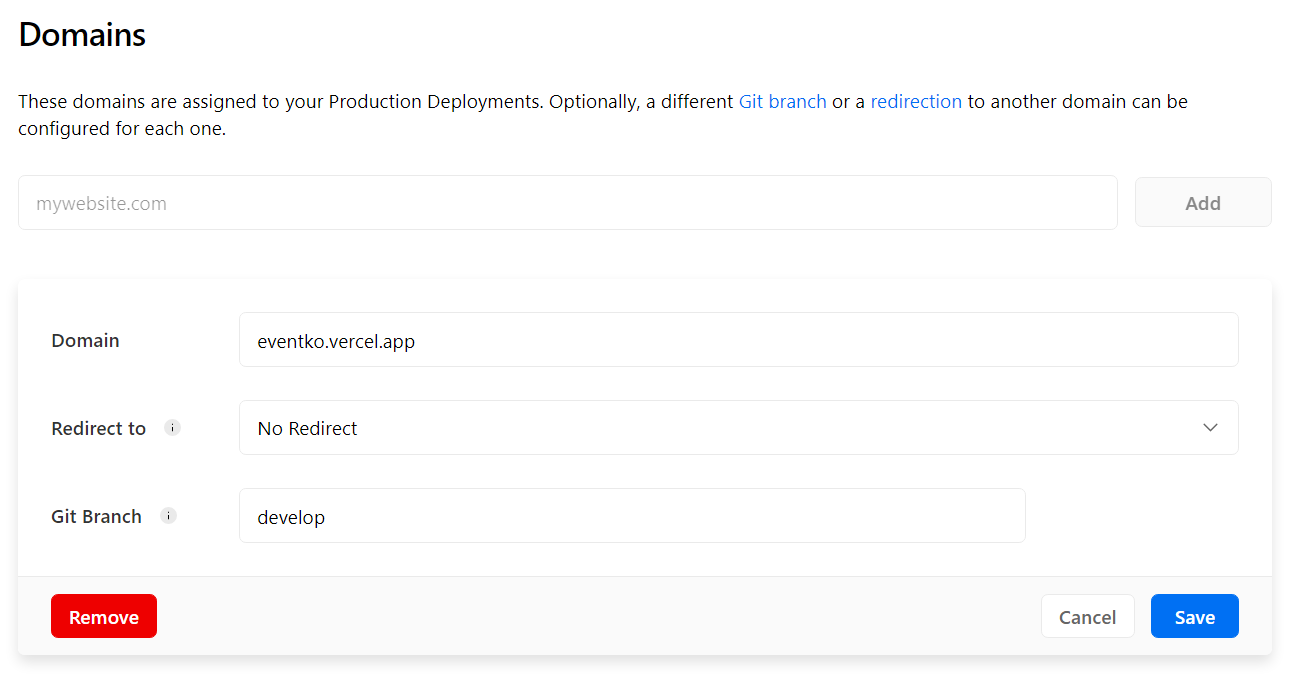
\includegraphics[width=\textwidth]{Opis deploymenta/Slika10.png}
					\caption{Promjena domene web-stranice}
				\end{figure}
			\end{packed_enum}
			
			\eject